\chapter{Conceitos básicos}
\label{cap:structure-of-speech}

Neste capítulo, abordaremos a parte teórica necessária para melhor entendimento e implementação do módulo no restante do trabalho. Em particular, veremos conceitos básicos de reconhecimento automático de voz e um pouco de sua implementação através do \emph{modelo oculto de Markov}.

% ---------------------------------------------------------------------

\section{Definição de reconhecimento de voz}

% https://en.wikipedia.org/wiki/Speech_recognition
% https://en.wikipedia.org/wiki/Computational_linguistics

\textit{Reconhecimento automático de voz} (ou da fala), ou \textit{speech to text} (STT), é um campo multidisciplinar que envolve as áreas de Inteligência Artificial, Estatística e Linguística. Busca-se desenvolver metodologias e tecnologias para que computadores sejam capazes de captar, reconhecer e traduzir a linguagem falada para texto.

A figura \ref{speech_system} apresenta os três componentes de um programa genérico STT: o usuário, o dispositivo que realiza o reconhecimento de voz e um \textit{software} de aplicação. O usuário codifica um comando através de sua voz; o dispositivo converte a mensagem falada para um formato interpretável; e o \textit{software} de aplicação aceita esta saída e realiza uma ação apropriada.

% https://www.nap.edu/read/19357/chapter/4#10
\begin{figure}[H]
  \centering
  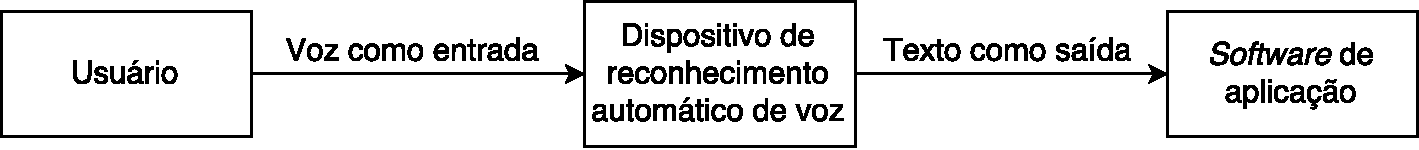
\includegraphics[width=.7\textwidth]{image/speech_system.pdf}
  \caption{Sistema genérico de reconhecimento automático de voz}
  \label{speech_system}
\end{figure}

% ---------------------------------------------------------------------

\subsection{História e aplicações}

% https://nexbridge.co.uk/speech-recognition-in-the-21st-century/
% https://www.callcentrehelper.com/the-top-five-uses-of-speech-recognition-technology-1536.htm
% http://www.pcworld.com/article/243060/speech_recognition_through_the_decades_how_we_ended_up_with_siri.html
O primeiro sistema de reconhecimento de voz conhecido foi o \textit{Audrey}, construído em 1952 por três pesquisadores do \textit{Bell Labs} para reconhecer dígitos falados por um único usuário. 10 anos depois, a IBM apresentou a máquina \textit{Shoebox}, que reconhecia 16 palavras em inglês.

Sistemas de reconhecimento de voz só tiveram um avanço realmente significativo na década de 80, devido a um método estatístico denominado \emph{modelo oculto de Markov} (HMM, sigla para \textit{Hidden Markov Model}). Ao invés de procurar por modelos de palavras em padrões de som, HMM considerava a probabilidade de um som desconhecido possuir palavras, o que acelerou o processo e tornou possível usar um vocabulário maior nos computadores. Outro modelo que ganhou bastante popularidade na época foi o de redes neurais, que é efetivo para classificar palavras isoladas e fonemas individuais mas encontra problemas em tarefas envolvendo reconhecimento contínuo. Ao contrário do HMM, este método não consegue modelar bem dependências temporais.

A evolução na tecnologia de reconhecimento de voz foi tamanha que, atualmente, é inegável seu impacto em nosso dia a dia. Um celular moderno consegue captar palavras ou pequenas frases de seu usuário dentre um enorme vocabulário para fazer buscas na Internet, tocar uma música ou fazer uma ligação. Muitas empresas utilizam máquinas para receber ligações de seus clientes; de acordo com o que interpretam, a chamada é redirecionada para um funcionário mais adequado. Alguns países chegam até a usar reconhecimento de voz para autenticar a identidade de alguém por telefone, com o objetivo de evitar fornecer dados pessoais pelo mesmo. Também há usos em transportes, na área médica e para fins educativos.

% ---------------------------------------------------------------------

\section{Parâmetros de reconhecimento de voz}

% https://www.nap.edu/read/19357/chapter/4#10
% http://www.voice-commands.com/103.htm
Há diversos tipos de parâmetros que caracterizam as capacidades de um sistema de reconhecimento de voz. Eles se subdividem nos três tipos a seguir.

% ---------------------------------------------------------------------

\subsection{Específicos ao aplicativo}

Relacionados a como o aplicativo em si realiza o reconhecimento de voz. Inclui dois parâmetros:

\begin{itemize}
\item A \textbf{forma de falar}, que pode ser através de \emph{palavras isoladas}, com pausas entre elas; \emph{palavras conectadas}, que são concatenadas sem pausas; ou \emph{fala contínua}, onde o fluxo de palavras é semelhante a uma fala natural.

\item \textbf{Existência de treinamento}, que subdivide aplicativos em dois grupos:

% https://speechangel.com/2016/05/04/difference-speaker-dependent-speaker-independent-recognition-software
\begin{itemize}[label=\small\bullet]
\item Os sistemas \emph{dependentes} (\textit{speaker-dependent}), caracterizados pelo \emph{treinamento} feito pelo usuário. Isto é, são computadores que analisam e se adaptam aos padrões particulares da fala captada, resultando em uma maior acurácia. Geralmente, o usuário deve ler algumas páginas de texto para a máquina antes de começar a usar o sistema. Esta variante é comumente usada em casos particulares, onde um número limitado de palavras deve ser reconhecido com bastante precisão.

\item Os sistemas \emph{independentes} (\textit{speaker-independent}), que são desenvolvidos para reconhecer a voz de qualquer pessoa e não requerem treinamento. É a melhor opção para aplicações interativas que usam voz, já que não é viável fazer com que os usuários leiam páginas de texto antes do uso. Sua desvantagem é a acurácia menor se comparado ao reconhecimento dependente; para contornar isso, costuma-se limitar o vocabulário reconhecido pelo sistema.
\end{itemize}

\end{itemize}

% ---------------------------------------------------------------------

\subsection{Específicos à tarefa}

Dependendo do objetivo a ser alcançado com o reconhecimento de voz, alguns parâmetros podem ser melhor ajustados para obter maior velocidade ou acurácia. São eles:

\begin{itemize}
\item O \textbf{vocabulário}, referente a quantas palavras são reconhecidas pelo sistema. O tamanho pode ser pequeno (menor que 20 palavras) até muito grande (mais de 20 mil palavras), sendo diretamente proporcional à velocidade do reconhecimento. Além disso, a similaridade entre a pronúncia de algumas palavras pode afetar a acurácia, uma vez que a distinção entre elas torna-se mais complicada.

\item A \textbf{sintaxe}, isto é, a gramática artificial que o sistema aceita para uma determinada tarefa. O exemplo mais simples seria uma máquina de estados finita, onde as palavras permitidas após um estado ou nó são definidas explicitamente.

\item O \textbf{fator de ramificação}, que é uma forma de medir a complexidade da sintaxe. É definido como o número médio de palavras permitidas em cada nó da gramática, e possui grande impacto sobre o desempenho do sistema.
\end{itemize}

% ---------------------------------------------------------------------

\subsection{Ambientais}

Dentre os vários parâmetros externos ao sistema e que podem interferir no reconhecimento de voz, destacam-se:

\begin{itemize}
\item A taxa \textbf{sinal-para-ruído}, que avalia a intensidade média do sinal recebido em relação ao ruído de fundo, tipicamente medido em decibéis (dB). Quanto menor a taxa, maior a dificuldade no reconhecimento de voz.

\item O \textbf{próprio usuário}, o que inclui o volume de sua voz, a velocidade com que fala e até mesmo sua condição psicológica (o nível de estresse de um piloto sob ataque em uma aeronave é diferente de alguém simplesmente querendo ouvir uma música).
\end{itemize}

% ---------------------------------------------------------------------

\section{Estrutura da fala}

% ---------------------------------------------------------------------

\section{Modelo oculto de Markov}
